% Created 2021-05-26 Wed 09:16
% Intended LaTeX compiler: pdflatex
\documentclass[smaller]{beamer}\usepackage{listings}
\usepackage{color}
\usepackage{amsmath}
\usepackage{array}
\usepackage[T1]{fontenc}
\usepackage{natbib}
\lstset{
keywordstyle=\color{blue},
commentstyle=\color{red},stringstyle=\color[rgb]{0,.5,0},
literate={~}{$\sim$}{1},
basicstyle=\ttfamily\small,
columns=fullflexible,
breaklines=true,
breakatwhitespace=false,
numbers=left,
numberstyle=\ttfamily\tiny\color{gray},
stepnumber=1,
numbersep=10pt,
backgroundcolor=\color{white},
tabsize=4,
keepspaces=true,
showspaces=false,
showstringspaces=false,
xleftmargin=.23in,
frame=single,
basewidth={0.5em,0.4em},
}
\usepackage{natbib, dsfont, pgfpages, tikz,amssymb, amsmath,xcolor}
\bibliographystyle{abbrvnat}
% New operators and commands
\newcommand{\Z}{\mathbb{Z}}
\newcommand{\Q}{\mathbb{Q}}
\newcommand{\R}{\mathbb{R}}
\newcommand{\N}{\mathbb{N}}
\newcommand{\C}{\mathbb{C}}
\renewcommand{\S}{\mathbb{S}}
\newcommand{\blank}{\makebox[1ex]{\textbf{$\cdot$}}}
\newcommand\independent{\protect\mathpalette{\protect\independenT}{\perp}}
\def\independenT#1#2{\mathrel{\rlap{$#1#2$}\mkern2mu{#1#2}}}
\renewcommand{\phi}{\varphi}
\renewcommand{\epsilon}{\varepsilon}
\newcommand*\diff{\mathop{}\!\mathrm{d}}
\newcommand{\weakly}{\rightsquigarrow}
\newcommand\smallO{
  \mathchoice
    {{\scriptstyle\mathcal{O}}}% \displaystyle
    {{\scriptstyle\mathcal{O}}}% \textstyle
    {{\scriptscriptstyle\mathcal{O}}}% \scriptstyle
    {\scalebox{.6}{$\scriptscriptstyle\mathcal{O}$}}%\scriptscriptstyle
}
\newcommand{\midd}{\; \middle|\;}
\newcommand{\1}{\mathds{1}}
\usepackage{ifthen} %% Empirical process with default argument
% \newcommand{\G}[1][]{%
%    \ifthenelse{ \equal{#1}{} }
%       {\ensuremath{\mathbb{G}_n}}
%       {\ensuremath{\mathbb{G}_{#1}}}
% }
% New version:
\newcommand{\G}[2][n]{
{\ensuremath{\mathbb{G}_{#1}}{\left[#2\right]}}
}
\DeclareMathOperator*{\argmin}{\arg\!\min}

% New operators for consistent notation
\newcommand{\V}{\mathrm{Var}} % variance
\newcommand{\measure}[1]{\mathrm{{#1}}} % measure
% \newcommand{\measure}[1]{\textnormal{\textbf{{#1}}}} % measure
\newcommand{\m}[1]{\measure{#1}} % measure shortcut
\newcommand{\eqd}{\stackrel{d}{=}} % equality in distribution
\newcommand{\arrow}[1]{\xrightarrow{\; {#1} \;}}
\newcommand{\arrowP}{\xrightarrow{\; \m{P} \;}} % convergence in probability
\newcommand{\leb}{\lambda} % the Lebesgue measure
\newcommand{\T}{\top} % transpose
\newcommand{\KL}{\ensuremath{D_{\mathrm{KL}}}}

\usepackage{xargs}
% Make it easy to change counterfactual notation:
\newcommandx{\cf}[4][3={}, 4={}]{
  % \ifthenelse{ \equal{#4}{} }
  % {{#1^{#2}}(#3)}
  {\ifthenelse{ \equal{#3}{} }
    {{#1^{#2}}_{#4}}
    {{#1^{#2}}_{#4}(#3)}}
}

% Easily change notation:
\DeclareMathOperator{\TT}{\Psi} % target parameter
\newcommand{\lp}{\mathcal{L}_{\P}^2} % shortcut for lp2 space
\newcommand{\empmeas}{\hat{\mathbb{P}}_n} % empirical measure
\DeclareMathOperator{\E}{\mathbb{E}} % expectation
\renewcommand{\P}{\m{P}} % probability
\newcommand{\ic}{\mathrm{IF}} % influence curve
\setbeamertemplate{footline}[frame number]
\beamertemplatenavigationsymbolsempty
\usepackage{appendixnumberbeamer}
\setbeamercolor{gray}{bg=white!90!black}

\renewcommand*\familydefault{\sfdefault}
\itemsep2pt
\usepackage[utf8]{inputenc}
\usepackage[T1]{fontenc}
\usepackage{graphicx}
\usepackage{grffile}
\usepackage{longtable}
\usepackage{wrapfig}
\usepackage{rotating}
\usepackage[normalem]{ulem}
\usepackage{amsmath}
\usepackage{textcomp}
\usepackage{amssymb}
\usepackage{capt-of}
\usepackage{hyperref}
\usetheme{default}
\author{Anders Munch}
\date{\today}
\title{Journal club -- undersmoothed HAL}
\begin{document}

\maketitle
\section{Setting: Estimation of the ATE and undersmoothing}
\label{sec:org6254a2d}

\begin{frame}[label={sec:orgf2d15cf}]{The article}
\begin{onlyenv}<1>
\begin{center}
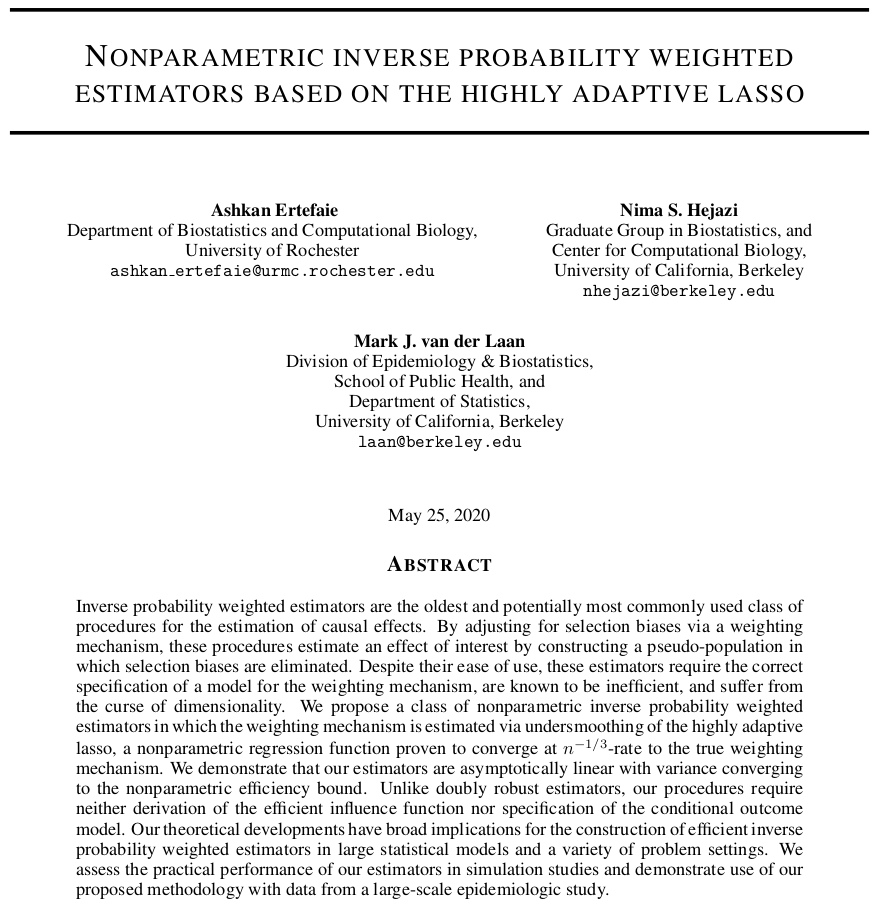
\includegraphics[width=0.75\textwidth]{./screenshots/abstract.png}
\end{center}
\end{onlyenv}

\begin{onlyenv}<2>
\begin{center}
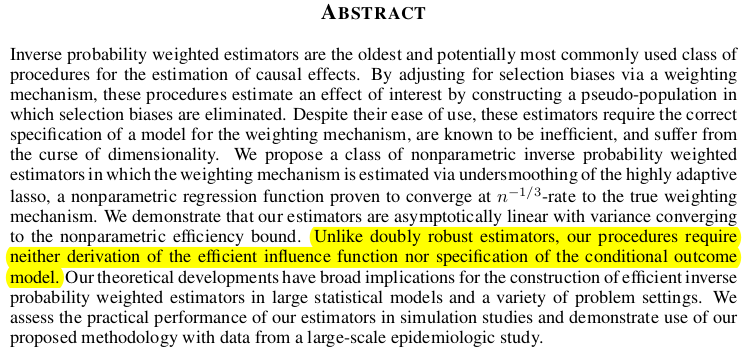
\includegraphics[width=0.9\textwidth]{./screenshots/abstract2.png}
\end{center}
\end{onlyenv}
\end{frame}


\begin{frame}[label={sec:org67d37da}]{Setting and notation -- the average treatment effect}
\begin{itemize}[<+->]
\item We observe \(n\) iid. samples from \(O = (W, A, Y) \sim P_0 \in \mathcal M\), where \(\mathcal M\)
is the nonparametric model.
\item \(W \in \mathcal W\) are baseline covariates, \(A \in \{0,1\}\) is treatment indicator, and \(Y\)
is the outcome of interest.
\item \(G \colon \mathcal M \rightarrow \mathcal G\) with \(\mathcal G := \{G(P) \, : \, P \in \mathcal
  M\}\) is the functional nuisance parameter \(G := G(P)\) denoting the treatment mechanism, i.e.,
\(G(P)(a \mid w) := \E_{P}(A=a \mid W=w)\).
\item We let \(Y^a\) denote the potential outcome under the intervention \(\mathrm{do}(A = a)\), and the
full data unit as \(X = (W, Y^0, Y^1) \sim P_X \in \mathcal M^F\).
\item The target parameter is \(\Psi^F \colon \mathcal M^F \rightarrow \R\), \(\Psi^F(P_X) :=
  \E_{P_X}(Y^1)\), i.e., the mean counterfactual outcome under treatment.
\item Under standard identification assumptions
\begin{equation*}
  \Psi^F(P_X) = \Psi(P) := \E_{P}[\E_{P}(Y \mid A=1, W)],
\end{equation*}
where \(\Psi\colon \mathcal M \rightarrow \R\).
\end{itemize}
\end{frame}

\begin{frame}[label={sec:org24311a0}]{Score functions and canonical gradient}
Score function using inverse probability weights:
\begin{equation*}
  U_G(O; \Psi) := \frac{AY}{G(1 \mid W)} - \Psi(P).
\end{equation*}
\pause Score function based on the canonical gradient
\begin{equation*}
  D^{\star}(O; P) := U_G(O; \Psi) - D_{\text{CAR}}(P),
\end{equation*}
where \(D_{\text{CAR}}(P) = \Pi(U_G(\Psi) \mid T_{\text{CAR}})\) is the projection onto the nuisance
tangent space \(T_{\text{CAR}}\). \pause The projection is given as
\begin{equation*}
  D_{\text{CAR}}(P) = \frac{A - G(A \mid W)}{G(A \mid W)}Q(1, W),
\end{equation*}
where \(Q(1, W) := \E_{P}(Y \mid A=1, W)\) is the conditional mean outcome \citep{robins1994estimation,van2003unified}.
\end{frame}


\begin{frame}[label={sec:orgb3a9318}]{Estimating the ATE -- solve a score function}
\pause
\begin{block}{Solve \(P_n[U_{G_n}] = 0\): The inverse probability weighted estimator}
\begin{equation*}
  \Psi(P_n, G_n) = \frac{1}{n}\sum_{i=1}^{n}\frac{A_iY_i}{G_n(A_i \mid W_i)}.
\end{equation*}
\pause
\end{block}
\begin{block}{Solve \(P_n[D^{\star}_{G_n, Q_n}] = 0\): The augmented IPW estimator}
\begin{equation*}
  \Psi^{\star}(P_n, G_n, Q_n) = \frac{1}{n}\sum_{i=1}^{n}\frac{A_iY_i}{G_n(A_i \mid W_i)} -
  \frac{A_i - G_n(A_i \mid W_i)}{G_n(A_i \mid W_i)}Q_n(1, W_i).
\end{equation*}

\hfill

\pause
\begin{description}[\leftmargin=1em]
\item[{\color{green}\(\checkmark\)}] Vanishing first order bias -- rate \(n^{-1/4}\) sufficient for \(G_n\)
and \(Q_n\) \pause
\item[{\color{red}\(\times\)}] Two nuisance parameters to estimate \pause
\item[{\color{red}\(\times\)}] Need to find the EIF
\end{description}
\end{block}
\end{frame}

\section{HAL}
\label{sec:org647380e}
\begin{frame}[label={sec:org211062e}]{The Highly Adaptive Lasso (HAL) -- nuisance estimator}
\begin{onlyenv}<2>
\(\mathbb{D}[0, \tau]\) is the Banach space of real-valued càdlàg functions on a cube \([0,\tau]
   \in \R^d\). For a function \(f \in \mathbb{D}[0, \tau]\) and a subset \(s \subset \{1, \dots, d\}\)
define
\begin{equation*}
  f_s \colon [0_s, \tau_s] \rightarrow \R, \quad f_s(u_s) := f(u_s, 0_{-s}),
\end{equation*}
where \(u_s = (u_j \, : \, j \in s)\) and \(u_{-s}\) is the complement of \(u_s\). 

\vfill

The sectional variation norm of a function \(f \in \mathbb{D}[0, \tau]\) is
\begin{equation*}
  \Vert f \Vert_{\nu}^{\star} := |f(0)| + \sum_{s \subset \{1, \dots, d \}}\int_{0_s}^{\tau_s}  |\diff f_s(u_s)|,
\end{equation*}
where the sum is over all subset of the coordinates \(\{1, \dots, d\}\).
\end{onlyenv}

\begin{onlyenv}<3>
\begin{center}
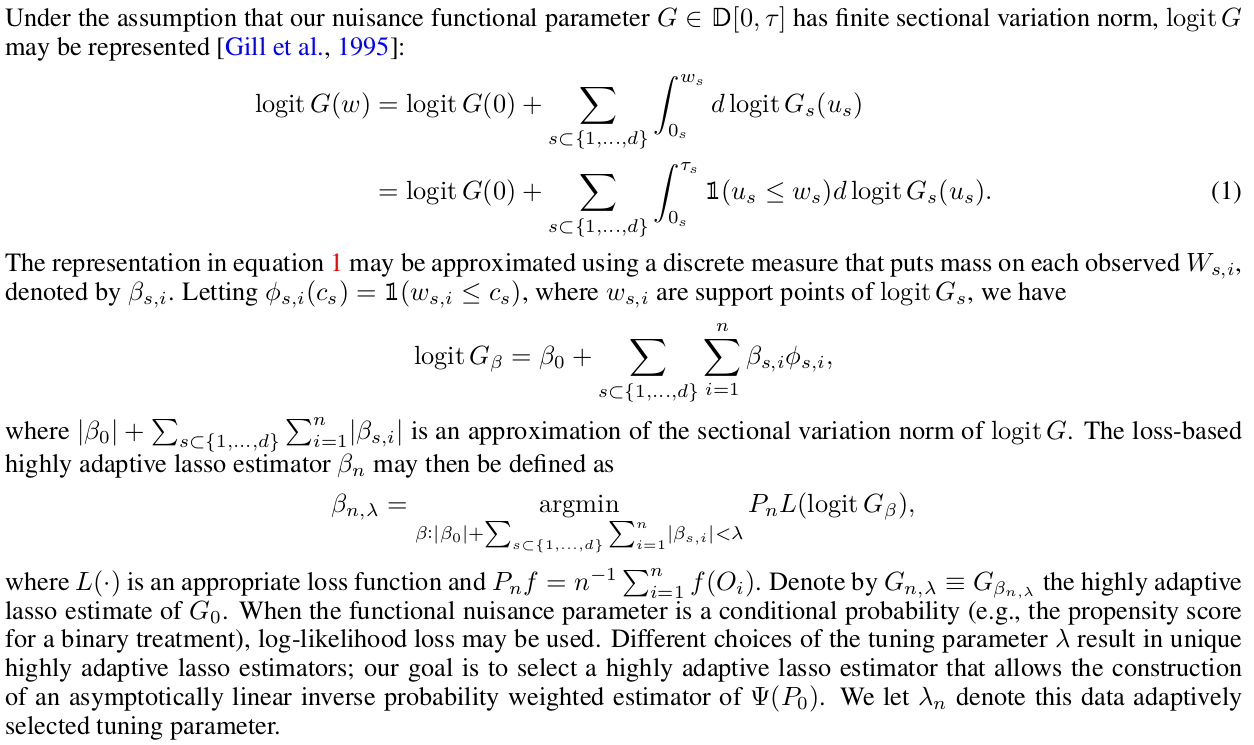
\includegraphics[width=1.03\textwidth]{./screenshots/hal.png}
\end{center}
\end{onlyenv}
\end{frame}

\begin{frame}[label={sec:org990e36d}]{The smoothing hyperparameter}
\begin{onlyenv}<1>
\color{white}     \center small \(\lambda \quad \quad \quad \quad \quad\) large
\begin{center}
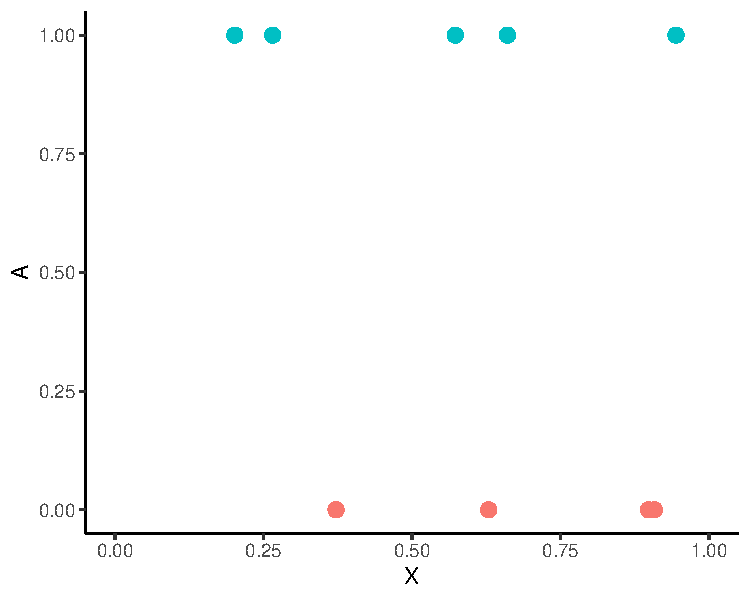
\includegraphics[width=.9\linewidth]{./hal-smoothing-dat.pdf}
\end{center}
\end{onlyenv}

\begin{onlyenv}<2>
\center small \(\quad \lambda \quad \quad \quad \quad \quad \quad\) large

\begin{center}
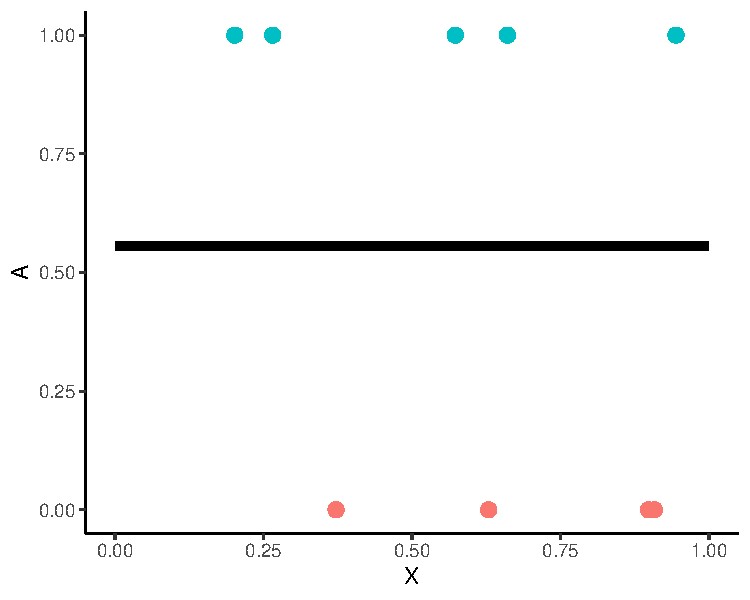
\includegraphics[width=.9\linewidth]{./hal-smoothing0.pdf}
\end{center}
\end{onlyenv}

\begin{onlyenv}<3>
\center small \(\quad \quad \lambda \quad \quad \quad \quad \quad\) large

\begin{center}
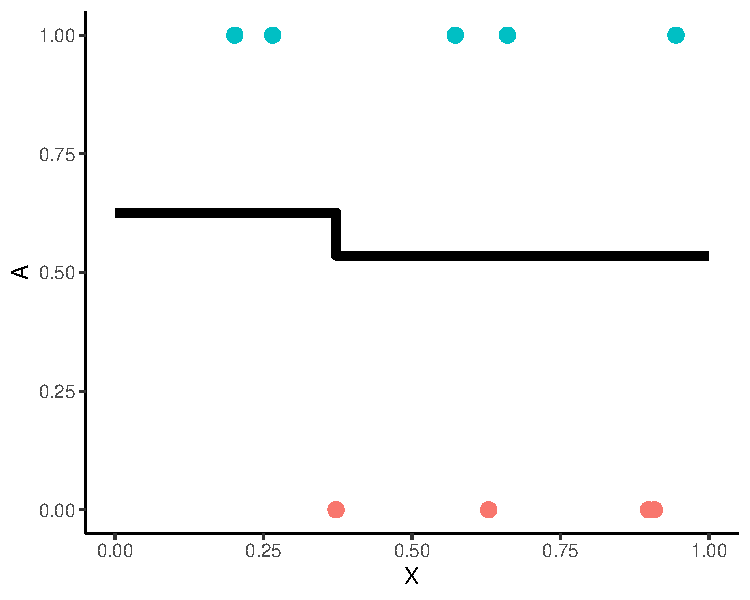
\includegraphics[width=.9\linewidth]{./hal-smoothing1.pdf}
\end{center}
\end{onlyenv}

\begin{onlyenv}<4>
\center small \(\quad \quad \quad  \lambda \quad \quad \quad \quad\) large

\begin{center}
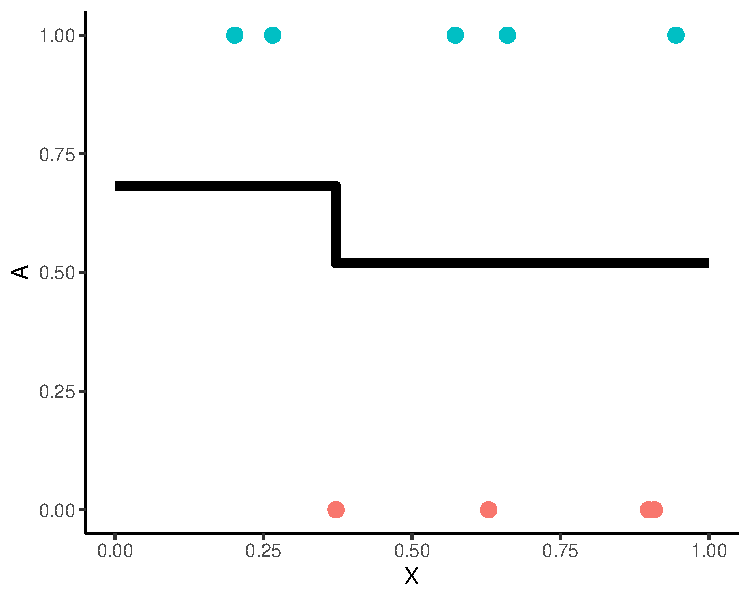
\includegraphics[width=.9\linewidth]{./hal-smoothing2.pdf}
\end{center}
\end{onlyenv}

\begin{onlyenv}<5>
\center small \(\quad \quad \quad \quad   \lambda \quad \quad \quad\) large

\begin{center}
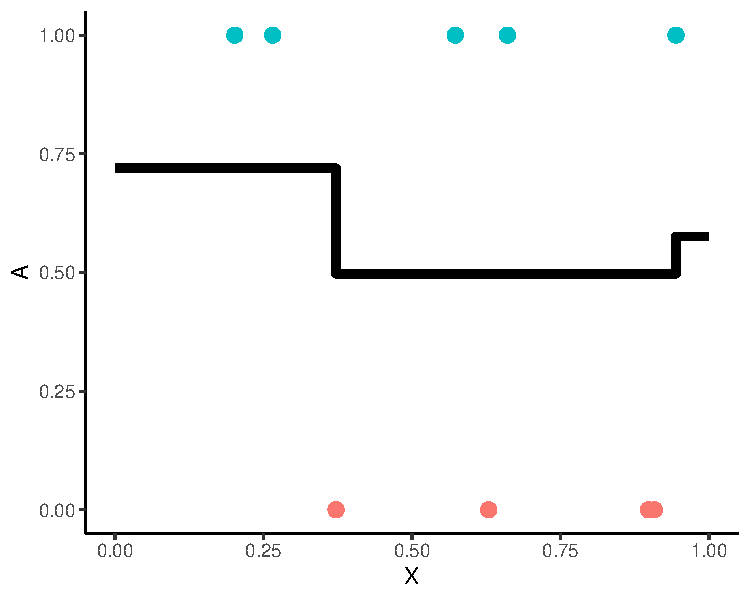
\includegraphics[width=.9\linewidth]{./hal-smoothing3.pdf}
\end{center}
\end{onlyenv}

\begin{onlyenv}<6>
\center small \(\quad \quad \quad \quad \quad   \lambda \quad \quad\) large

\begin{center}
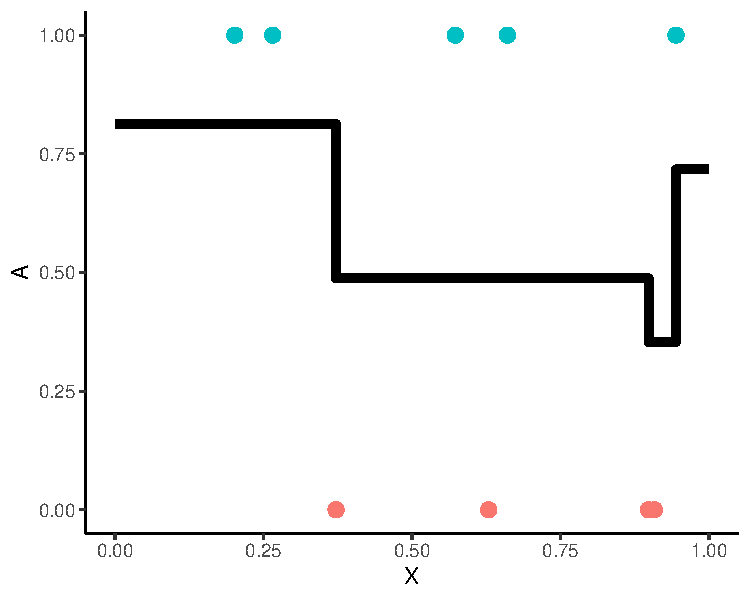
\includegraphics[width=.9\linewidth]{./hal-smoothing4.pdf}
\end{center}
\end{onlyenv}

\begin{onlyenv}<7>
\center small \(\quad \quad \quad \quad \quad \quad   \lambda \quad\) large

\begin{center}
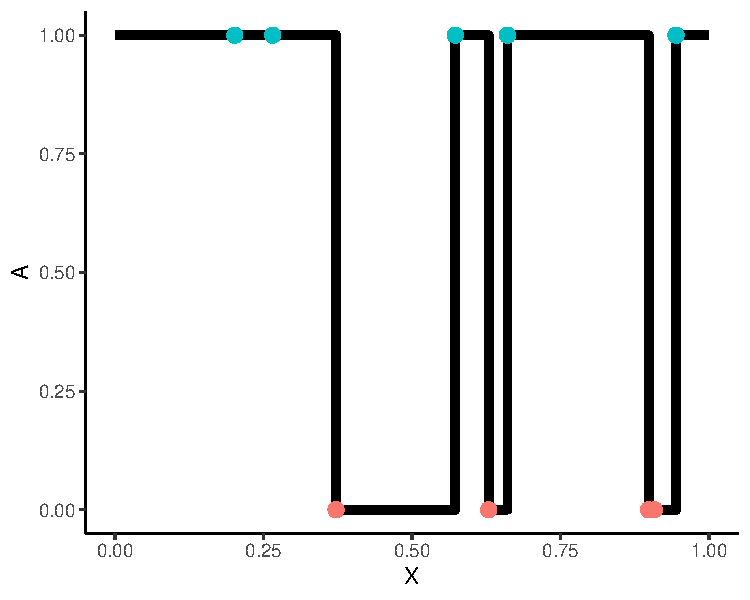
\includegraphics[width=.9\linewidth]{./hal-smoothing5.pdf}
\end{center}
\end{onlyenv}
\end{frame}

\begin{frame}[label={sec:orged9d0c1}]{Properties of the HAL estimator}
\begin{itemize}[<+->]
\item Only assumption is that the target function is càdlàg with finite sectional variation norm.
\item Converges at rate faster than \(n^{-1/4}\) regardless of the dimension \(d\) of the covariate
space; specifically, at rate \(n^{-1/3} \log(n)^{d/2}\) \citep{van2017uniform,van2017generally}.
\item Belongs to a Donsker function class.
\item We can use cross-validation to select the penalization/smoothing parameter \(\lambda\).
\end{itemize}

\begin{block}<5->{Undersmoothed HAL}
Using CV we find the choice of \(\lambda\) which gives the optimal bias-vaiance trade-off with
respect to the \emph{nuisance parameter}. \pause We want instead to pick the hyperparamter \(\lambda\)
to get the correct bias-vaiance trade-off with respect to the \emph{target parameter} \pause
\(\rightarrow\) undersmooth the HAL estimator.

\hfill

\pause Old-school knowledge that undersmoothing is needed in other similar settings (density
estimation)
\citep{laurent1996efficient,goldstein1996efficient,bickel2003nonparametric,goldstein1992optimal}.
\end{block}
\end{frame}

\begin{frame}[label={sec:orgadeffa5}]{Undersmoothing}
\begin{onlyenv}<1>
\center Optimizing the nuisance estimator
\begin{center}
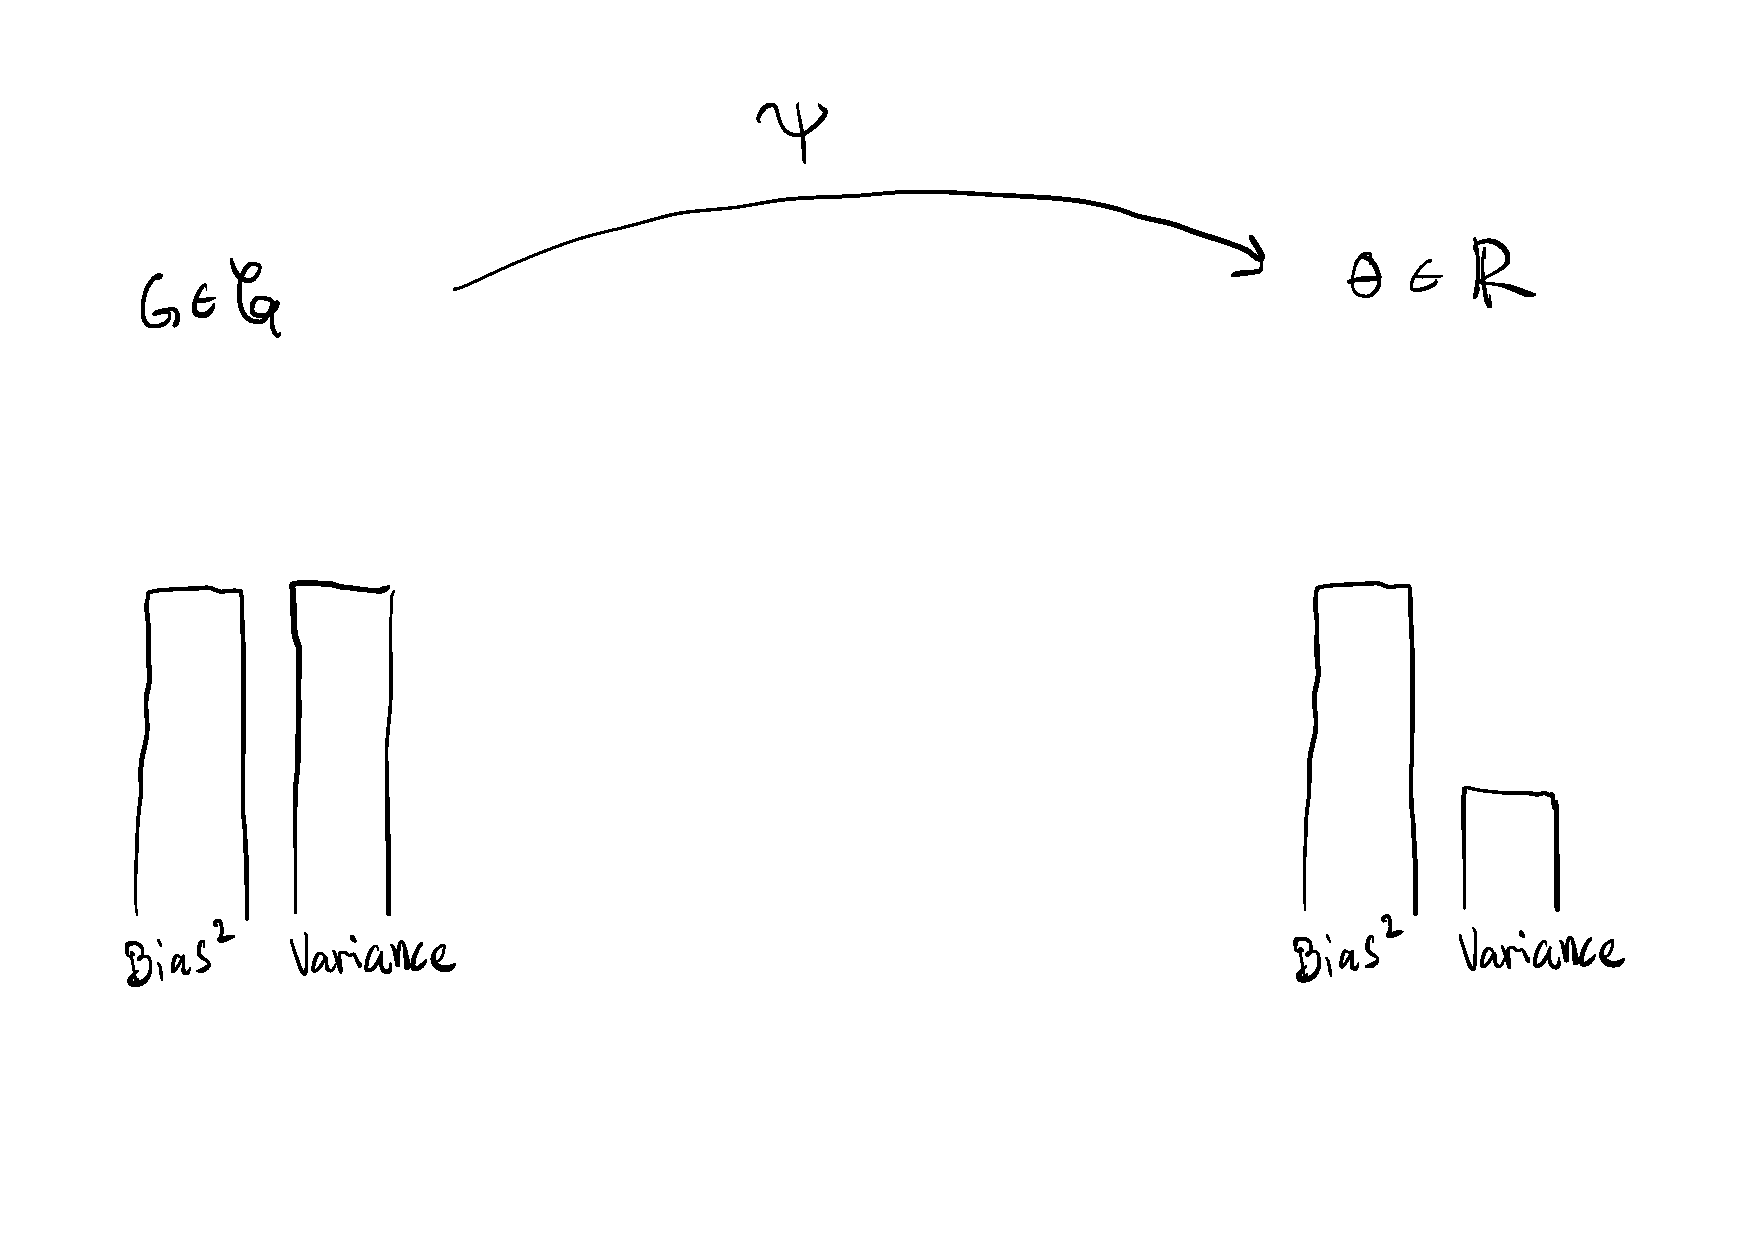
\includegraphics[width=1\textwidth]{./Undersmooth-tradeoff1.pdf}
\end{center}
\end{onlyenv}

\begin{onlyenv}<2>
\center Undersmoothing the nuisance estimator
\begin{center}
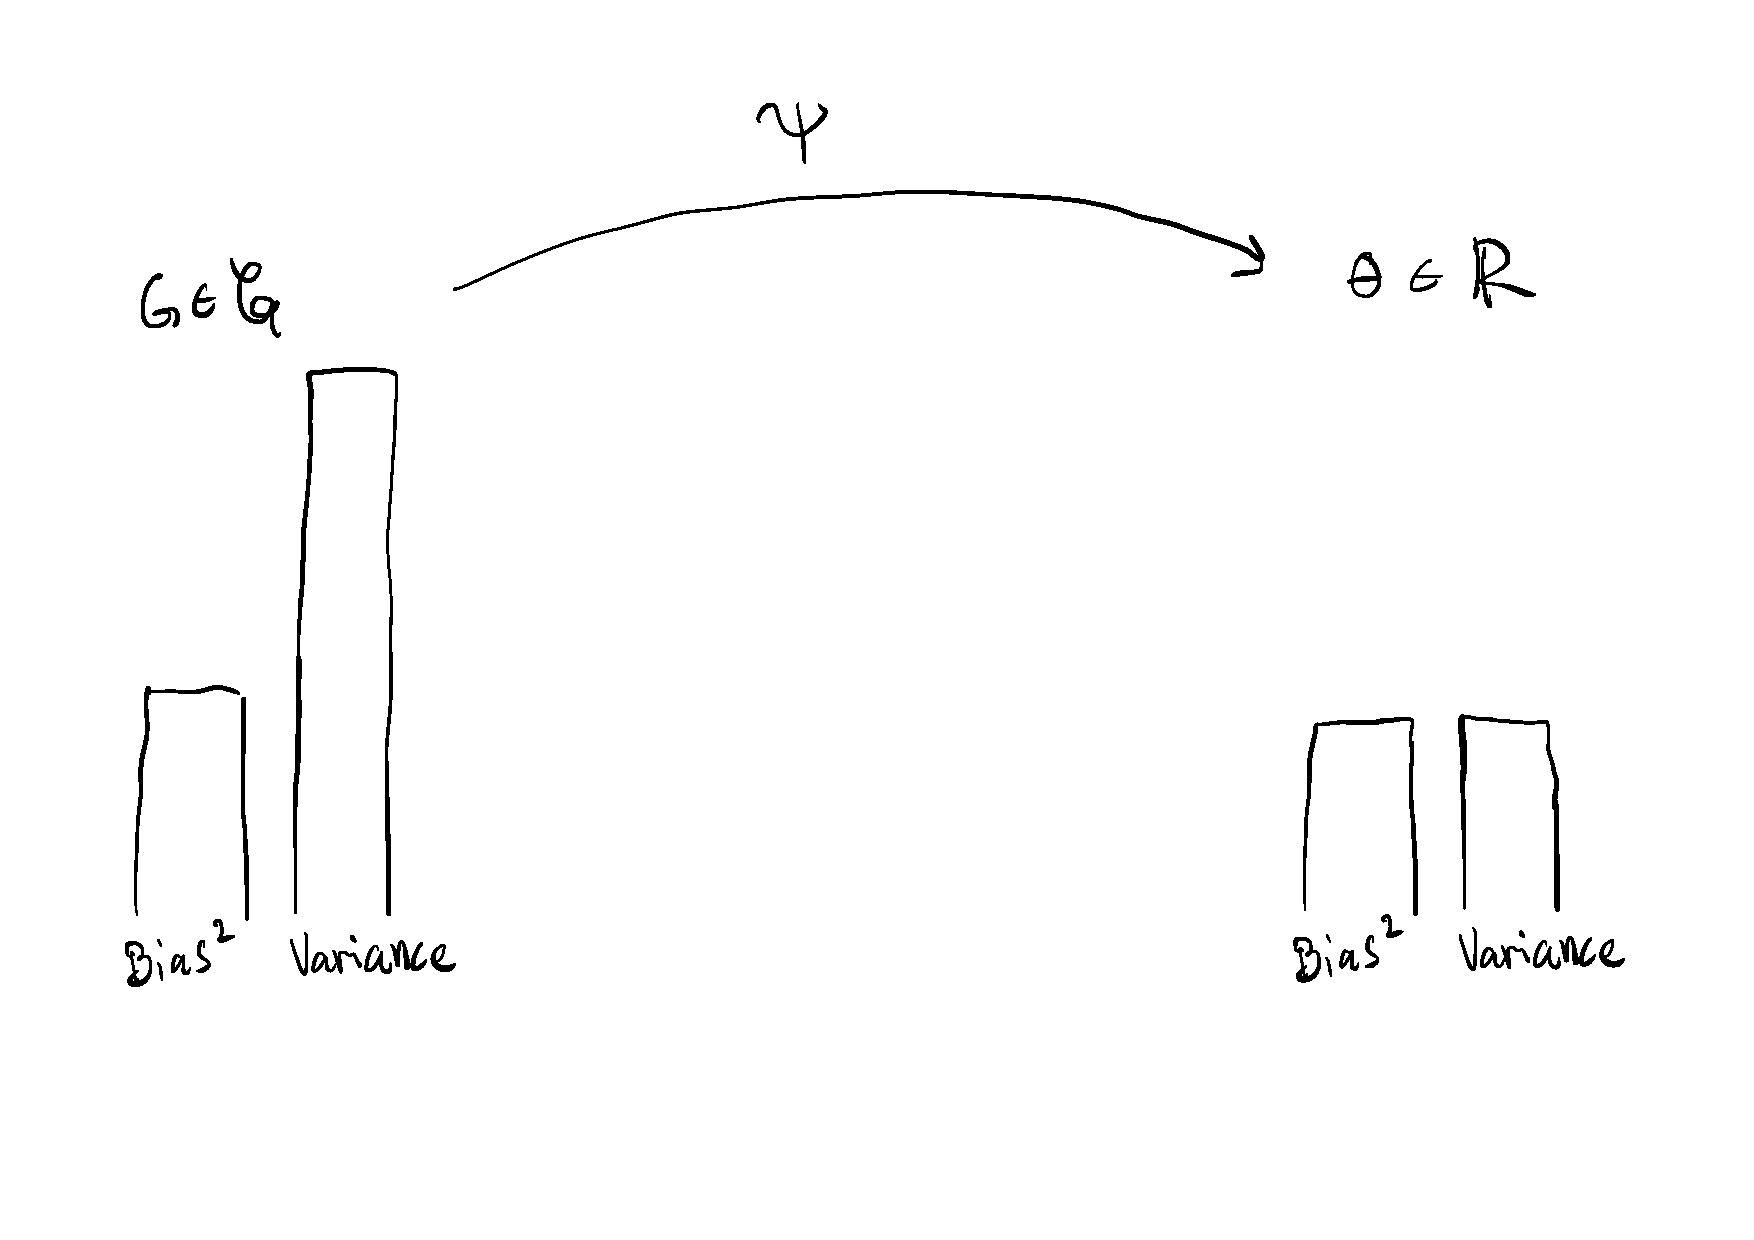
\includegraphics[width=1\textwidth]{./Undersmooth-tradeoff2.pdf}
\end{center}
\end{onlyenv}
\end{frame}

\section{Undersmoothed HAL}
\label{sec:orgf291186}
\begin{frame}[label={sec:org2d04721}]{Undersmoothing in theory}
\pause
\begin{theorem}[Lemma 1 and Theorem 1 of the article]
Let \(G_{n,\lambda_n}\) be a HAL estimator of \(G_0\) with $\lambda_n$ chosen to satisfy
\begin{equation}
  \label{eq:1}
  \min_{(s,j) \in \mathcal{J}_n}\left\Vert P_n 
  \left[
    \frac{\partial }{\partial \epsilon} L(\mathrm{logit} G_{n, \lambda_n} + \epsilon \phi_{s,j}) 
  \right] 
\right\Vert = \smallO_P(n^{- \frac 1 2}),
\end{equation}
where $L(\blank)$ is the log-likelihood loss and $\mathcal{J}_n$ is a set of indices for the basis
functions such that $\beta_{n,j,s} \not = 0$. Then the (IPW) estimator
\begin{equation*}
  \Psi(P_n, G_{n, \lambda_n}) = \frac{1}{n}\sum_{i=1}^{n}\frac{A_iY_i}{G_{n,\lambda_n}(A_i \mid W_i)}
\end{equation*}
is asymptotically efficient. \pause
\end{theorem}

\begin{proof}[Sketch of proof:]
Use empirical process theory and convergence rates of HAL to write
\begin{equation*}
  \Psi(P_n, G_{n, \lambda_n}) - \Psi(P_0, G_0) = P_n[D^{\star}]
  - P_n[D_{\text{CAR}}(Q_0, G_0, G_{n,\lambda_n})] + \smallO_P(n^{- \frac 1 2})
\end{equation*}
\pause Lemma 1 states that \eqref{eq:1} implies \(P_n[D_{\text{CAR}}(Q_0, G_0, G_{n,\lambda_n})] =
\smallO_P(n^{- \frac 1 2})\)
\end{proof}
\end{frame}

\begin{frame}[label={sec:org340365a}]{Undersmoothing in practice}
\pause

\begin{onlyenv}<2>
\begin{center}
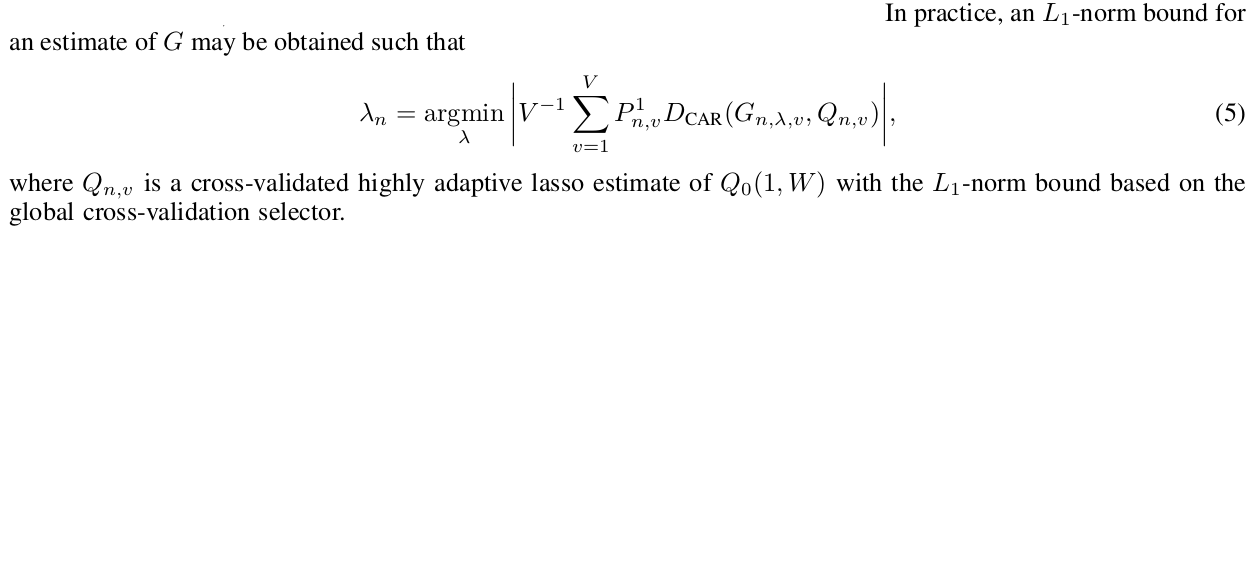
\includegraphics[width=1.02\textwidth]{./screenshots/undersmoothing-practice0.png}
\end{center}
\end{onlyenv}

\begin{onlyenv}<3->
\begin{center}
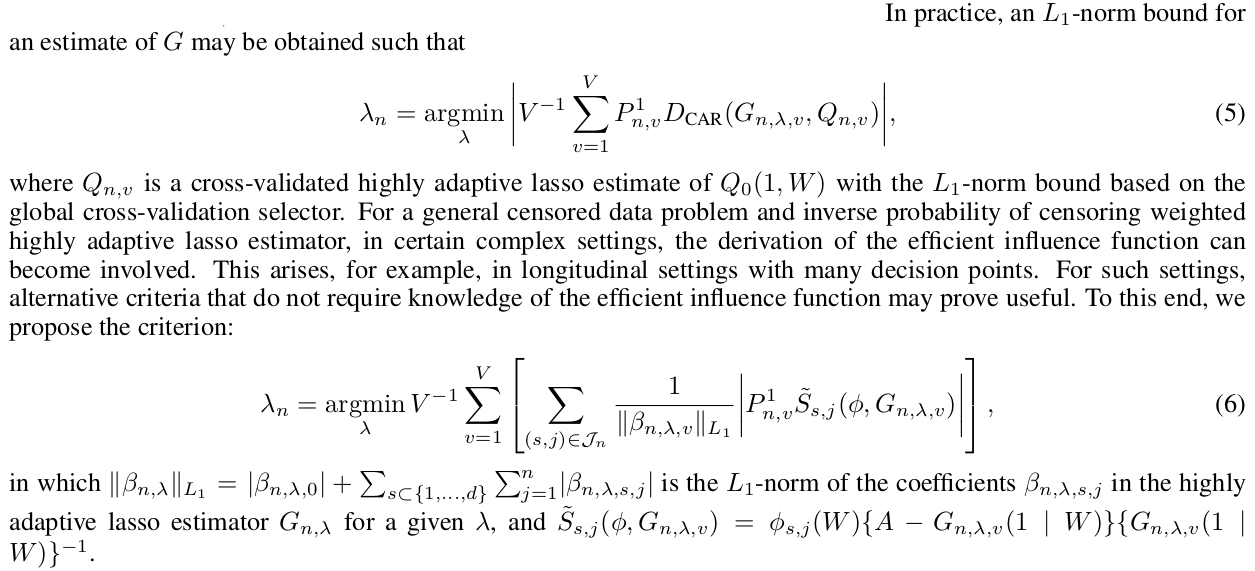
\includegraphics[width=1.02\textwidth]{./screenshots/undersmoothing-practice1.png}
\end{center}
\end{onlyenv}

\begin{block}<4->{\color{red} But no theoretical results about this in the article}
No proof that this achieves the theoretical undersmoothing rate\ldots{}?
\end{block}
\end{frame}

\section{Numerical studies (and application)}
\label{sec:org0c7d9e6}
\begin{frame}[label={sec:org84cb2a9}]{Numerical studies:}
\begin{center}
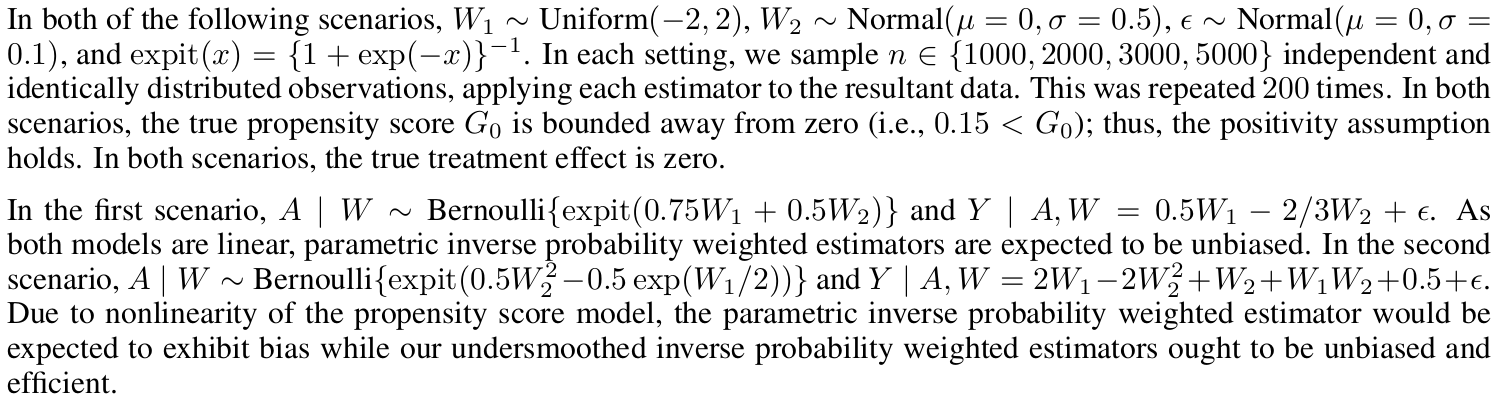
\includegraphics[width=1\textwidth]{./screenshots/numerical-results.png}
\end{center}

\begin{description}
\item[{Scenario 1}] Correctly specified parametric model
\item[{Scenario 2}] Mis-specified parametric model
\end{description}
\end{frame}

\begin{frame}[label={sec:org3a8cc58}]{Scenario 1: Correctly specified parametric model}
\begin{center}
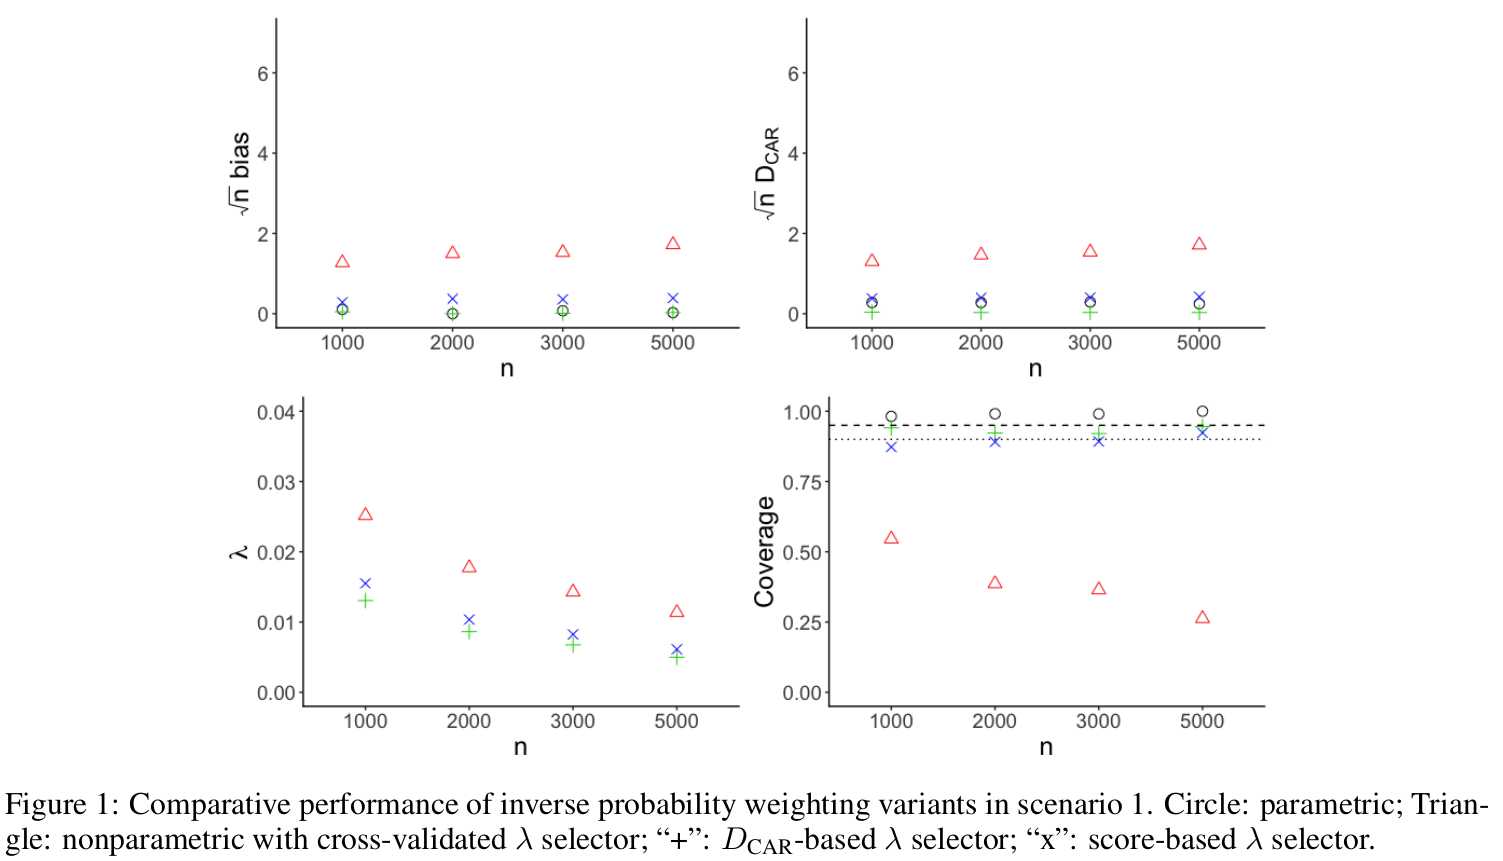
\includegraphics[width=1\textwidth]{./screenshots/scenario1.png}
\end{center}

\begin{block}<2>{\color{red} Coverage\ldots{} how?}
No variance estimator?
\end{block}
\end{frame}

\begin{frame}[label={sec:org113addb}]{Scenario 2: Mis-specified parametric model}
\begin{center}
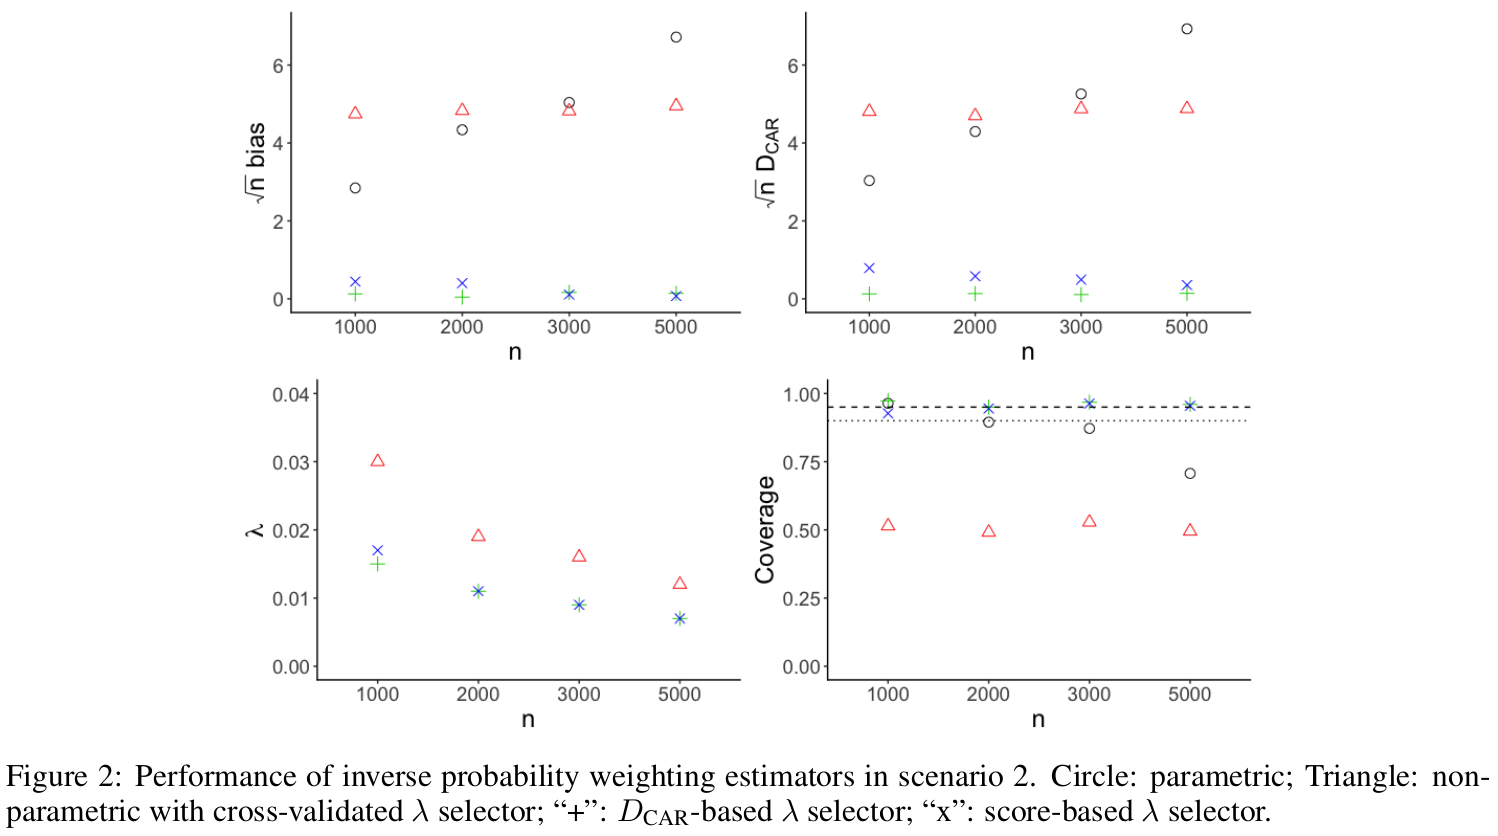
\includegraphics[width=1\textwidth]{./screenshots/scenario2.png}
\end{center}
\end{frame}

\section{Thoughts and perspective}
\label{sec:orgd4fb3d3}
\begin{frame}[label={sec:orgc68e53d}]{Perspective, thoughts, summary, and discussion}
\begin{block}{Perspective}
\begin{itemize}
\item Nice to not need to find the EIF. Probably not so important for the ATE but potentially for more
complex problems.
\item Spend computational energy on optimizing the right bias-variance trade-off.
\item Could be nice to generalize to other nuisance estimators. These might not achieve \(n^{-1/4}\)
convergence in high-dimensions, so undersmoothing could be needed even when using the EIF.
\end{itemize}
\pause
\end{block}
\begin{block}{Thoughts}
\begin{itemize}
\item No theoretical result for how to do undersmoothing in practice.
\item Variance estimator???
\end{itemize}
\pause
\end{block}
\begin{block}{Questions and comments?}
\end{block}
\end{frame}
\section{References}
\label{sec:orga92c697}
\bibliography{/home/amnudn/Documents/latex/default-bib.bib}
\end{document}